% REALM 2026 short paper using the official ACL review style.
\documentclass[11pt]{article}
\usepackage[review]{acl}
\usepackage{times}
\usepackage{latexsym}
\usepackage{booktabs}
\usepackage{graphicx}
\usepackage{amssymb}
\usepackage[T1]{fontenc}
\usepackage[utf8]{inputenc}
\usepackage{microtype}

\title{Do Multi-Hop RAG Evaluations Measure Agentic Behavior?\\A Failure-Mode Audit}

\author{Anonymous \\ Submission to REALM 2026}

\begin{document}
\maketitle

\begin{abstract}
Modern multi-hop retrieval-augmented generation (RAG) systems decide \emph{what} to retrieve,
\emph{when} to stop, and \emph{how} to recover, but their evaluations may not measure this control
behavior. We audit a documented, purposive corpus of 32 iterative, graph-based, and agentic multi-hop
RAG papers across 10 outcome, process, and cost signals. Repeat coding of a seeded, stratified 22\%
sample gives 97.1\% agreement (pooled Cohen's $\kappa=0.93$). Within this corpus, 97\% report
final-answer accuracy, 13\% joint evidence completeness, and 3\% retrieval-control quality; no
iterative/agentic paper reports recovery (0/15), and no tool-agent reports tool-error rate (0/5).
We turn recurring failure modes into an operational table linking trigger,
observable signal, consequence, recovery, and detecting metric, plus a practitioner checklist. A
retrieval-only illustration over all 22,398 multi-support questions in the official 2Wiki, MuSiQue,
and HotpotQA development splits shows joint evidence completeness 8--31 points below aggregate
recall@20. Rather than another architecture survey, this is a transparent audit showing that
systems with iterative or agentic components are usually scored on endpoints, not their control behavior.
\end{abstract}

\section{Introduction}
Multi-hop question answering (QA) requires assembling several interdependent facts into a reasoning
chain. RAG has responded with a progression of designs: dense and late-interaction retrievers, graph
systems that traverse entity relations, iterative retrieve-then-reason loops, and tool-using agents
that plan their own retrieval. A recurring narrative motivates this progression: a set of
\emph{failure modes} (silent retrieval failures, context fragmentation, broken graph paths, cascading
errors from a wrong hop) that each new design claims to mitigate through more agentic control over
retrieval.

These failure modes are behavioral: they concern \emph{how} a system retrieves, decides to stop, and
recovers, not merely whether the final answer string matches. If a system is agentic, its evaluation
should expose process quality. We ask a simple, falsifiable question: \textbf{do multi-hop RAG
evaluations measure the retrieval-control behavior that iterative and agentic designs introduce?}

We answer with a quantitative audit rather than another narrative survey. We assemble a documented,
purposive corpus of 32
iterative, graph-based, and agentic multi-hop RAG papers through a documented protocol and code each
for whether it reports a set of outcome, agent-quality, and cost signals
(\S\ref{sec:method}). We then (i) recast the standard failure taxonomy as an \emph{operational} table
that maps each trigger to the observable signal and metric that would catch it
(\S\ref{sec:failuremodes}); (ii) quantify how often each signal is actually reported
(\S\ref{sec:findings}); and (iii) distill a practitioner checklist
(\S\ref{sec:checklist}).

Recent surveys catalog RAG \emph{methods} and reasoning
strategies~\citep{gao2023survey,rag_reasoning_survey_2025,agentic_rag_survey_2026}. Our focus differs:
we audit \emph{evaluation practice}. Our contributions are:
\begin{itemize}\itemsep0pt
  \item A transparent coding protocol and appendix matrix auditing multi-hop RAG evaluation (32 papers,
  10 dimensions, with a repeat-coding consistency audit on 22\% of the sample).
  \item An operational failure-mode table (trigger $\to$ signal $\to$ consequence $\to$ recovery $\to$
  metric) that turns descriptive limitations into measurable quantities.
  \item Quantified reporting gaps showing process-level signals are rarely reported in this sample, and a
  checklist tying task properties to the retrieval strategy and the metrics to report.
  \item A full-split retrieval illustration (2Wiki, MuSiQue, HotpotQA; 22,398 questions) showing that
  the omitted evidence-completeness metric exposes an 8--31 point gap, with larger gaps as the number
  of required passages grows.
\end{itemize}

\section{Method}
\label{sec:method}
\paragraph{Corpus construction.} We searched arXiv and the ACL/EMNLP/NAACL and NeurIPS/ICLR/SIGIR
proceedings (2020--2026) using queries combining ``multi-hop'' with \{RAG, retrieval-augmented,
iterative retrieval, agentic retrieval, graph RAG, knowledge-graph QA\}. We constructed a purposive
sample covering four design families and several influential adjacent systems whose evaluations
include retrieval-like tool use or multi-step control. The corpus contains iterative decomposition
(10), tool-using agents (5), graph-based reasoning (15), and iterative dense retrieval (2). It is
intended to characterize reporting practice across these families, not to estimate architecture
prevalence in the full literature. Appendix~\ref{app:corpus} gives the full list, source links, and
per-paper codes.

\paragraph{Coding scheme.} For each paper we read the evaluation section and code, as $1/0/?$ (reported
/ not reported / unclear), the dimensions in Table~\ref{tab:dims}: two \emph{outcome} signals, five
\emph{agent-quality} signals, and three \emph{cost} signals. We coded conservatively: a dimension is
$1$ only when the paper reports a corresponding quantitative measure. To keep judgments defensible we
pre-specified conventions before final reconciliation, e.g.: aggregate recall@$k$ that credits
\emph{partial} support is
\emph{not} evidence completeness (A1 requires a joint/all-support metric such as joint passage-set EM);
``retrieval frequency'' (fraction of steps that trigger retrieval) counts as retrieval use/calls (C1);
offline indexing time alone does not count as latency (C3). For trajectory correctness (A4), a
quantified manual error analysis over a stated sample counts, while isolated examples do not.

\paragraph{Consistency check.} With seed 20260803 we sampled seven papers, stratified as two iterative,
one agentic, three graph, and one dense system. A source-verification pass re-coded all 70 cells before
reconciliation. Raw agreement was 68/70 (97.1\%) and pooled Cohen's $\kappa=0.93$. The two source-resolved
disagreements corrected MDR's trajectory code and HippoRAG~2's latency code.
Appendix~\ref{app:corpus} reports both code matrices and the sample rule.

\begin{table}[t]\centering\footnotesize
\caption{Coding dimensions. Agent-quality signals (A) are the behaviors that distinguish an agent from
a static pipeline.}
\label{tab:dims}
\begin{tabular}{@{}ll@{}}
\toprule
\textbf{Group} & \textbf{Dimension} \\
\midrule
Outcome (S) & answer EM/F1/acc; retrieval recall@$k$ \\
\midrule
Agent (A) & evidence completeness (joint support) \\
 & retrieval-control decision quality \\
 & failed-retrieval recovery \\
 & trajectory / path correctness \\
 & tool-error rate \\
\midrule
Cost (C) & retrieval use/calls; tokens/cost; latency \\
\bottomrule
\end{tabular}
\end{table}

\section{Failure Modes as Observable Signals}
\label{sec:failuremodes}
The literature's failure modes are usually stated descriptively. Table~\ref{tab:operational} recasts
them operationally: each trigger produces an observable signal, has a downstream consequence, and admits a
recovery action. Crucially, each trigger maps to a metric that would \emph{detect} it. The rightmost column
is what we audit for in \S\ref{sec:findings}; every row names the measurement that operationalizes it.

\begin{table*}[t]\centering\footnotesize
\caption{Operational failure-mode table for multi-hop RAG. Each descriptive failure becomes a
measurable quantity (rightmost column). A/S/C refer to the coding dimensions in Table~\ref{tab:dims}.}
\label{tab:operational}
\begin{tabular}{@{}p{2.6cm}p{2.65cm}p{2.5cm}p{2.55cm}p{2.25cm}@{}}
\toprule
\textbf{Failure trigger} & \textbf{Observable signal} & \textbf{Downstream consequence} & \textbf{Recovery action} & \textbf{Detecting metric} \\
\midrule
Embedding bottleneck (silent retrieval failure) & gold passage ranked low / missed despite plausible top-$k$ & incomplete evidence; confident wrong answer & query reformulation; multi-vector / late interaction & evidence recall@$k$; joint support recall (S2/A1) \\
\midrule
Context fragmentation & a required fact split across chunks; one piece absent & broken reasoning chain & semantic chunking; neighbor expansion & evidence completeness (A1) \\
\midrule
Premature / late stopping (iterative) & loop halts before all hops, or over-retrieves & missing evidence or wasted budget & sufficiency check; adaptive stop & control-decision quality (A2); retrieval calls (C1) \\
\midrule
Failed / wrong intermediate hop & a hop returns wrong or empty evidence & later hops condition on bad evidence (cascade) & backtrack; re-query; verification & recovery rate (A3); trajectory correctness (A4) \\
\midrule
Shortcut reasoning (right answer, wrong path) & answer correct but support unused / spurious & brittle, non-generalizing behavior & path supervision; distractor stress test & trajectory correctness (A4) \\
\midrule
Tool / action-call error (agentic) & malformed query or failed tool call & dropped or corrupted step & error handling; retries & tool-error rate (A5) \\
\midrule
Graph construction gaps / missing edges & reasoning path halts at an absent edge & unreachable evidence & edge completion; hybrid fallback & support recall on reachable golds (S2/A1) \\
\bottomrule
\end{tabular}
\end{table*}

\section{Findings: The Reporting Gap}
\label{sec:findings}
Table~\ref{tab:findings} and Figure~\ref{fig:gap} report the fraction of the 32 systems that measure
each dimension. The pattern is stark. Final-answer accuracy is nearly universal (97\%), and retrieval
recall is common (44\%). But the agent-quality signals that the failure modes in
Table~\ref{tab:operational} call for are rarely measured: evidence completeness 13\%, retrieval-control
quality 3\%, and trajectory correctness 16\%. Using relevant family denominators, only 1/15 iterative
or agentic papers reports control quality, none reports failed-retrieval recovery, and none of the five
explicitly tool-using agents reports tool-error rate. Even the near misses quantify retrieval
\emph{use}, such as Toolformer's call frequency and FrugalRAG's search count/cost~\citep{toolformer,frugalrag},
rather than failure or recovery rates. Cost signals are reported unevenly (calls 38\%, tokens 41\%, latency 41\%),
and disproportionately by the subset of papers whose contribution
\emph{is} efficiency.

\begin{table}[t]\centering\small
\caption{Corpus-wide reporting rate per dimension (fixed denominator 32). Family-relevant denominators
for control, recovery, and tool errors are reported in the text.}
\label{tab:findings}
\begin{tabular}{@{}llr@{}}
\toprule
\textbf{Group} & \textbf{Dimension} & \textbf{Reported} \\
\midrule
Outcome & answer EM/F1/acc & 31/32 (97\%) \\
 & retrieval recall@$k$ & 14/32 (44\%) \\
\midrule
Agent & evidence completeness & 4/32 (13\%) \\
 & retrieval-control quality & 1/32 (3\%) \\
 & failed-retrieval recovery & \textbf{0/32 (0\%)} \\
 & trajectory correctness & 5/32 (16\%) \\
 & tool-error rate & \textbf{0/32 (0\%)} \\
\midrule
Cost & retrieval use / calls & 12/32 (38\%) \\
 & tokens / cost & 13/32 (41\%) \\
 & latency & 13/32 (41\%) \\
\bottomrule
\end{tabular}
\end{table}

\begin{figure}[t]\centering
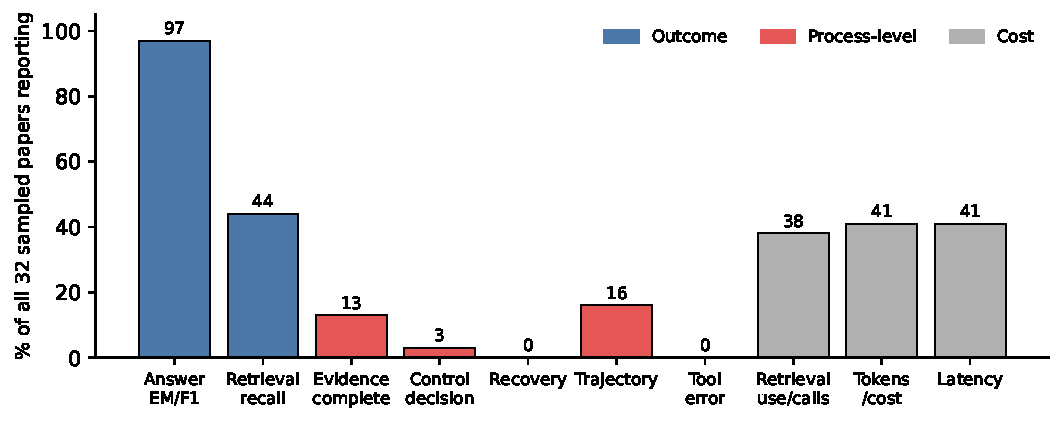
\includegraphics[width=\columnwidth]{fig_reporting_gap.pdf}
\caption{Percentage of the 32 systems reporting each signal. Outcome metrics dominate; agent-quality
signals (recovery, tool-error, retrieval control, evidence completeness) remain sparse.}
\label{fig:gap}
\end{figure}

\paragraph{Where the exceptions are.} The few agent-quality measurements are instructive.
\emph{Evidence completeness} is measured by only four systems, all via a joint/all-support metric:
MDR's joint two-passage recall~\citep{mdr}, HippoRAG's All-Recall@$k$~\citep{hipporag}, Beam
Retrieval's joint gold-passage-set EM~\citep{beam_retrieval}, and LinearRAG's all-necessary-information
Evidence Recall~\citep{linearrag}; every other retrieval-reporting system
uses aggregate recall@$k$ that credits partial support. \emph{Retrieval-control quality} is measured
by exactly one system: Adaptive-RAG's question-complexity router~\citep{adaptive_rag}, whose $\sim$54.5\%
routing accuracy exposes a control-policy oracle gap. This is a query-level routing decision rather
than a per-hop stop test, so we use the broader control-quality label. Five papers expose trajectory
quality: Think-on-Graph reports path overlap with ground-truth relation paths~\citep{think_on_graph};
Self-Ask~\citep{self_ask}, IRCoT~\citep{ircot}, ReAct~\citep{react}, and MDR~\citep{mdr} report quantified
manual analyses. Two boundary cases sharpen the point: GraphRAG
reports \emph{no} answer accuracy at all~\citep{graphrag} (LLM-judge win-rates on an incomparable
summarization axis), and StepChain~\citep{stepchain} leaves uncertainty-aware re-decomposition,
backtracking, and sub-question robustness metrics to future work, closely matching the gaps we quantify.

\paragraph{Interpretation.} Systems are scored on the endpoint, not the behavior. A system can obtain
high answer EM while stopping at the wrong hop, failing to recover, or traversing an incorrect
path. These failures need not surface under endpoint-only reporting. This is precisely the concern REALM
raises for agents: without process-level metrics, agentic control is credited or blamed on outcome
alone, and claims of ``adaptive'' or ``self-corrective'' behavior go unvalidated.

\section{Empirical Illustration}
\label{sec:experiment}
To show that the audited gap matters, we use BGE-large-en-v1.5~\citep{bge} on the complete official
development splits of 2Wiki~\citep{2wiki}, MuSiQue~\citep{musique}, and
HotpotQA~\citep{hotpotqa}. For each split we deduplicate the union of its provided candidate contexts,
then perform exact dense ranking. We report aggregate recall@20 (mean gold-passage recall) versus joint
recall@20 (all gold passages retrieved), with paired 95\% bootstrap intervals (5,000 resamples).
Appendix~\ref{app:experiment} gives the protocol and support-count breakdown.

\begin{table}[t]\centering\small
\caption{Exact retrieval on all official multi-support development questions. $\Delta$ is the paired
aggregate-minus-joint gap; brackets give its 95\% bootstrap interval.}
\label{tab:exp}
\begin{tabular}{@{}lrrr@{}}
\toprule
\textbf{Dataset ($n$)} & \textbf{agg.} & \textbf{joint} & \textbf{$\Delta$ [95\% CI]} \\
\midrule
2Wiki (12,576) & 73.2 & 45.3 & 27.9 [27.5, 28.4] \\
MuSiQue (2,417) & 65.5 & 34.6 & 30.9 [29.8, 32.0] \\
HotpotQA (7,405) & 91.0 & 82.7 & 8.3 [7.9, 8.8] \\
\bottomrule
\end{tabular}
\end{table}

The divergence is not an artifact of mixing two- and four-support questions. On two-support subsets,
the gaps remain 21.0 points (2Wiki), 22.0 (MuSiQue), and 8.3 (HotpotQA). It then widens sharply with
the required evidence set: for four-support 2Wiki questions, aggregate recall is 53.4\% while joint
recall is only 0.7\%; for four-support MuSiQue, the corresponding values are 42.8\% and 3.0\%.
The median \emph{weakest-link} rank is 3 on HotpotQA but 48 on 2Wiki and 56 on MuSiQue.

A fixed two-pass feedback control (query plus top-1 passage, fused by reciprocal-rank
fusion~\citep{rrf}) does not repair the gap. At @20 it changes aggregate recall by $-4.0$, $-4.0$,
and $-0.4$ points and joint recall by $-2.9$, $-1.9$, and $-0.2$ on 2Wiki, MuSiQue, and HotpotQA,
respectively; the paired joint interval includes zero only for HotpotQA. Thus a plausible expansion
can look only mildly harmful under aggregate recall while losing substantially more complete evidence
sets. Both effects are invisible without the completeness signal that only 13\% of the audited sample reports.

\section{A Practitioner Checklist}
\label{sec:checklist}
The audit yields actionable guidance. Table~\ref{tab:checklist} ties task properties to a retrieval
strategy and identifies the minimal metric set that would expose its characteristic failure mode. It shows
what to report \emph{beyond} answer accuracy.

\begin{table}[t]\centering\small
\caption{Choosing and evaluating a retrieval strategy. The metric column lists what to report beyond
answer accuracy to detect the strategy's dominant failure mode.}
\label{tab:checklist}
\begin{tabular}{@{}p{2.1cm}p{2.2cm}p{2.35cm}@{}}
\toprule
\textbf{Task property} & \textbf{Strategy} & \textbf{Report also} \\
\midrule
single-hop, high-recall corpus & static dense / hybrid top-$k$ & recall@$k$ \\
multi-hop, bounded hops, text & iterative retrieve-reason & evidence completeness; \#calls \\
multi-hop, entity/KB-centric & graph traversal & support recall; path correctness \\
open-ended, variable hops, tools & agentic planning & control/stop quality; recovery; tool errors; cost \\
\bottomrule
\end{tabular}
\end{table}

\section{Related Work}
Surveys of RAG and reasoning organize the field by
\emph{method}~\citep{gao2023survey,rag_reasoning_survey_2025,agentic_rag_survey_2026}. We are
complementary and narrower: a quantitative audit of \emph{evaluation practice} for multi-hop RAG, in
the spirit of reproducibility and reporting-standard studies. To our knowledge, prior surveys have
not quantified process-level metric reporting across iterative, graph, and agentic multi-hop RAG with
a paper-level coding matrix.

\section{Limitations}
The purposive, citation-skewed corpus yields descriptive rather than population estimates, and binary
codes compress partial reporting. Seven-paper repeat coding supports pooled but not stable dimension-wise
$\kappa$. The illustration uses one encoder, split-induced corpora, and fixed feedback, so it diagnoses
metrics rather than architectures. Logging actions is inexpensive, but judging control or recovery correctness
requires task-specific supervision.

\section*{Use of AI}
Generative AI assisted literature retrieval and drafting; the authors remain responsible.

\bibliography{references_realm}

\appendix
\section{Corpus and Coding Sheet}
\label{app:corpus}
Table~\ref{tab:corpus-codes} reports all 32 systems and all 10 reconciled codes. Paper names link to
the source used for coding. Families are I (iterative), T (tool-using agent), G (graph), and D
(iterative dense retrieval). Within each bit string, positions follow Table~\ref{tab:dims}; 1 means
reported and 0 means not reported.

\begin{center}
\footnotesize
\captionof{table}{Complete paper-level coding matrix. S=\{S1,S2\}, A=\{A1,...,A5\}, and C=\{C1,C2,C3\}.
Each linked system name opens the source version used for coding.}
\label{tab:corpus-codes}
\setlength{\tabcolsep}{4pt}
\begin{tabular}{@{}lcccc@{}}
\toprule
\textbf{System} & \textbf{F} & \textbf{S} & \textbf{A} & \textbf{C} \\
\midrule
\href{https://arxiv.org/abs/2210.03350}{Self-Ask} & I & \texttt{10} & \texttt{00010} & \texttt{010} \\
\href{https://arxiv.org/abs/2212.10509}{IRCoT} & I & \texttt{11} & \texttt{00010} & \texttt{000} \\
\href{https://arxiv.org/abs/2212.14024}{DSP} & I & \texttt{10} & \texttt{00000} & \texttt{000} \\
\href{https://arxiv.org/abs/2205.10625}{Least-to-Most} & I & \texttt{10} & \texttt{00000} & \texttt{000} \\
\href{https://arxiv.org/abs/2305.15294}{ITER-RETGEN} & I & \texttt{11} & \texttt{00000} & \texttt{110} \\
\href{https://arxiv.org/abs/2305.06983}{FLARE} & I & \texttt{10} & \texttt{00000} & \texttt{100} \\
\href{https://arxiv.org/abs/2310.11511}{Self-RAG} & I & \texttt{10} & \texttt{00000} & \texttt{100} \\
\href{https://arxiv.org/abs/2403.14403}{Adaptive-RAG} & I & \texttt{10} & \texttt{01000} & \texttt{101} \\
\href{https://aclanthology.org/2025.emnlp-main.1011/}{RaDeR} & I & \texttt{11} & \texttt{00000} & \texttt{000} \\
\href{https://arxiv.org/abs/2501.05366}{Search-o1} & I & \texttt{10} & \texttt{00000} & \texttt{000} \\
\href{https://arxiv.org/abs/2210.03629}{ReAct} & T & \texttt{10} & \texttt{00010} & \texttt{000} \\
\href{https://arxiv.org/abs/2302.04761}{Toolformer} & T & \texttt{10} & \texttt{00000} & \texttt{100} \\
\href{https://arxiv.org/abs/2507.07634}{FrugalRAG} & T & \texttt{11} & \texttt{00000} & \texttt{111} \\
\href{https://www.ifaamas.org/Proceedings/aamas2025/pdfs/p50.pdf}{SCMRAG} & T & \texttt{10} & \texttt{00000} & \texttt{000} \\
\href{https://arxiv.org/abs/2602.03442}{A-RAG} & T & \texttt{10} & \texttt{00000} & \texttt{010} \\
\href{https://arxiv.org/abs/2404.16130}{GraphRAG} & G & \texttt{00} & \texttt{00000} & \texttt{010} \\
\bottomrule
\end{tabular}
\end{center}

\newpage
\begin{center}
\footnotesize
\textbf{Table~\ref{tab:corpus-codes} (continued).}\\[0.4em]
\setlength{\tabcolsep}{4pt}
\begin{tabular}{@{}lcccc@{}}
\toprule
\textbf{System} & \textbf{F} & \textbf{S} & \textbf{A} & \textbf{C} \\
\midrule
\href{https://arxiv.org/abs/2405.14831}{HippoRAG} & G & \texttt{11} & \texttt{10000} & \texttt{011} \\
\href{https://arxiv.org/abs/2502.14802}{HippoRAG2} & G & \texttt{11} & \texttt{00000} & \texttt{011} \\
\href{https://arxiv.org/abs/2405.20139}{GNN-RAG} & G & \texttt{11} & \texttt{00000} & \texttt{110} \\
\href{https://arxiv.org/abs/2307.07697}{Think-on-Graph} & G & \texttt{10} & \texttt{00010} & \texttt{100} \\
\href{https://arxiv.org/abs/2407.10805}{ToG-2} & G & \texttt{10} & \texttt{00000} & \texttt{101} \\
\href{https://aclanthology.org/2025.naacl-long.449/}{KG2RAG} & G & \texttt{11} & \texttt{00000} & \texttt{111} \\
\href{https://arxiv.org/abs/2507.08445}{Clue-RAG} & G & \texttt{10} & \texttt{00000} & \texttt{110} \\
\href{https://arxiv.org/abs/2503.10150}{HiRAG} & G & \texttt{10} & \texttt{00000} & \texttt{011} \\
\href{https://arxiv.org/abs/2412.15272}{SimGRAG} & G & \texttt{11} & \texttt{00000} & \texttt{001} \\
\href{https://arxiv.org/abs/2212.00959}{UniKGQA} & G & \texttt{11} & \texttt{00000} & \texttt{000} \\
\href{https://arxiv.org/abs/2510.02827}{StepChain} & G & \texttt{10} & \texttt{00000} & \texttt{001} \\
\href{https://arxiv.org/abs/2510.10114}{LinearRAG} & G & \texttt{11} & \texttt{10000} & \texttt{011} \\
\href{https://arxiv.org/abs/2502.12442}{HopRAG} & G & \texttt{11} & \texttt{00000} & \texttt{111} \\
\href{https://arxiv.org/abs/2412.06206}{SiReRAG} & G & \texttt{10} & \texttt{00000} & \texttt{001} \\
\href{https://arxiv.org/abs/2009.12756}{MDR} & D & \texttt{11} & \texttt{10010} & \texttt{001} \\
\href{https://arxiv.org/abs/2308.08973}{Beam-Retrieval} & D & \texttt{11} & \texttt{10000} & \texttt{000} \\
\bottomrule
\end{tabular}

\vspace{0.8em}
\captionof{table}{Paired repeat-coding matrix in S1,S2,A1--A5,C1--C3 order. The seeded,
family-stratified sample has 68/70 matching cells; the two changes shown in bold were resolved from
the cited sources before the corpus totals were computed.}
\label{tab:repeat-codes}
\setlength{\tabcolsep}{2.5pt}
\begin{tabular}{@{}llcc@{}}
\toprule
\textbf{System} & \textbf{Family} & \textbf{Initial pass} & \textbf{Verification pass} \\
\midrule
FLARE & iterative & \texttt{1000000100} & \texttt{1000000100} \\
IRCoT & iterative & \texttt{1100010000} & \texttt{1100010000} \\
Toolformer & tool-agent & \texttt{1000000100} & \texttt{1000000100} \\
SimGRAG & graph & \texttt{1100000001} & \texttt{1100000001} \\
HippoRAG2 & graph & \texttt{110000001\textbf{0}} & \texttt{110000001\textbf{1}} \\
GNN-RAG & graph & \texttt{1100000110} & \texttt{1100000110} \\
MDR & dense & \texttt{11100\textbf{0}0001} & \texttt{11100\textbf{1}0001} \\
\bottomrule
\end{tabular}
\end{center}

\clearpage

\section{Retrieval Illustration Protocol}
\label{app:experiment}
We use the official 2Wiki development split (12,576 questions), MuSiQue answerable development split
(2,417), and HotpotQA distractor validation split (7,405). Every question has at least two mapped
support passages. The split-induced corpora are the title--text-deduplicated unions of provided candidate
contexts: 56,661, 21,099, and 66,581 passages, respectively. Source revisions and SHA-256 checksums are
asserted before evaluation.

BGE-large-en-v1.5 is pinned to model revision \texttt{d4aa6901...e09}; queries use its documented
retrieval instruction.
Normalized vectors are ranked by exact inner product. The fixed feedback query is the normalized sum of
the original query and its top-1 passage; two depth-100 rankings are fused by RRF ($k_0=60$). We evaluate
@10 and @20, use 5,000 paired bootstrap resamples (seed 20260803), and apply exact paired McNemar tests to
joint-recall changes. Weakest-link ranks are exact to depth 2,000 and right-censored thereafter. We stored
one record per query and independently reconstructed every point estimate and paired contingency cell.

\begin{center}
\begin{minipage}{\columnwidth}
\small
\captionof{table}{Single-shot recall@20 stratified by required support count. The aggregate metric increasingly
masks incomplete evidence sets as the number of required passages grows.}
\label{tab:support-strata}
\centering
\begin{tabular}{@{}lrrrr@{}}
\toprule
\textbf{Dataset} & \textbf{Supports} & $n$ & \textbf{Aggregate} & \textbf{Joint} \\
\midrule
2Wiki & 2 & 9,825 & 78.7 & 57.7 \\
2Wiki & 4 & 2,751 & 53.4 & 0.7 \\
MuSiQue & 2 & 1,252 & 73.2 & 51.2 \\
MuSiQue & 3 & 760 & 64.9 & 24.2 \\
MuSiQue & 4 & 405 & 42.8 & 3.0 \\
HotpotQA & 2 & 7,405 & 91.0 & 82.7 \\
\bottomrule
\end{tabular}
\end{minipage}
\end{center}

\end{document}
